\documentclass[11pt,a4paper]{article}

\usepackage[utf8]{inputenc}
\usepackage[T1]{fontenc}
\usepackage{amsmath,amssymb,amsthm,mathtools}
\usepackage{geometry}
\usepackage{booktabs}
\usepackage{array}
\usepackage{graphicx}
\usepackage{hyperref}
\usepackage{xcolor}
\usepackage{float}

\geometry{margin=0.92in}
\hypersetup{
  colorlinks=true,
  linkcolor=blue!70!black,
  citecolor=blue!70!black,
  urlcolor=blue!70!black
}

\newtheorem{theorem}{Theorem}[section]
\newtheorem{proposition}[theorem]{Proposition}
\newtheorem{finding}[theorem]{Empirical Finding}
\theoremstyle{definition}
\newtheorem{definition}[theorem]{Definition}
\theoremstyle{remark}
\newtheorem{remark}[theorem]{Remark}

\title{\textbf{Multiway Hypergraph Rewriting, McKay Individualization--Refinement Canonicalization, and Rule Reducibility in Regenerative Morphospace}\\[0.55em]
\large Exact Isomorphism Compression, $44{,}534\times$ Quotient Exploration, Bioelectric Branching, and Machine-Checked Lean~4 Proofs Across \texttt{PlanformDB~2.5.0} and \texttt{LimbformDB~2.1.0}}

\author{
  \textbf{Joel Dietz}$^{1}$ \quad and \quad \textbf{Richard Assar}$^{2,*}$\\[0.35em]
  \small $^{1}$Infinite Morphospace \& Project Delphi Research Initiative (\texttt{https://github.com/fractastical/morpholib})\\
  \small $^{2}$Wolfram Institute (\texttt{https://github.com/WolframInstitute/HypergraphRewritingEngine})\\
  \small $^{*}$Proposed co-author (pending author review and approval)
}

\date{October 24, 2026}

\begin{document}
\maketitle

\begin{abstract}
Regenerative biology possesses two benchmark graph-encoded repositories of experimentally induced anatomical form: \textbf{PlanformDB~2.5.0} (Lobo, Malone \& Levin 2013, encoding $369$ planarian morphologies across $1{,}181$ anatomical regions) and \textbf{LimbformDB~2.1.0} (Lobo et al.\ 2014, encoding $555$ salamander, frog, crustacean, insect, and arachnid limb morphologies across $3{,}146$ joints). Until now, these databases have been treated primarily as static descriptive catalogs or target tables for continuous differential-equation fits. Conversely, the \textbf{Wolfram Physics Project} has recently produced a lock-free, model-checked C++20/CUDA multiway double-pushout (DPO) hypergraph rewriting engine (\texttt{WolframInstitute/HypergraphRewritingEngine}, \texttt{v1.0.0-rc2}; Assar 2026) featuring exact McKay-style individualization--refinement (IR) canonicalization, quotient exploration (\texttt{ExploreFromCanonicalStatesOnly}) with exact automorphism-orbit event/causal/branchial reconstruction, keyed transition weighting (\texttt{RuleWeights}), and per-state discrete differential geometry (\texttt{state\_geometry\_core.hpp}).

Here we bridge these two research programs by coupling the standalone C++20 \texttt{hg\_evolve} engine directly to \texttt{PlanformDB~2.5.0} and \texttt{LimbformDB~2.1.0} over Wolfram Exchange Format (WXF) and verifying the governing algebraic invariants in the \textbf{Lean~4} theorem prover (\texttt{0 sorry}). We report five principal findings:
\begin{enumerate}
  \item \textbf{Exact McKay IR Isomorphism Compression \& Discovery of Seven Hidden Topological Isomers in \texttt{PlanformDB}:} McKay IR canonicalization compresses the $369$ encoded planarian morphologies into exactly \textbf{$38$ canonical region-link isomorphism classes} ($9.7105\times$ redundancy, Shannon class entropy $2.3098\text{ bits}$; $126$ classes when Eye, Brain, Pharynx, and VNC organ hyperedges are attached) and compresses the $555$ \texttt{LimbformDB} morphologies into \textbf{$51$ canonical segment-tree classes} ($10.8824\times$ redundancy, entropy $3.5650\text{ bits}$; $92$ classes with digits). Crucially, exact IR canonicalization resolves \textbf{$7$ hidden topological isomers} in \texttt{PlanformDB} that are indistinguishable under standard $(\text{Head}, \text{Trunk}, \text{Tail}, \text{Links})$ region-count vectors ($31$ count buckets $\to 38$ IR classes), such as separating the $4$-region signature $(2\text{H}, 1\text{Tr}, 1\text{Ta}, 3\text{L})$ into radial Trunk-hub stars (\texttt{\#3 Side head}, $n=12$, First Zagreb invariant $Z_1 = 12$), Head-hub stars (\texttt{\#112}, $n=1$), and linear intercalary chains (\texttt{\#119 Head on head}, $n=2$, $Z_1 = 10$).
  \item \textbf{Three-Tier DPO Regeneration Grammar \& Algebraic Reducibility to a Three-Rule Primitive Basis $\mathcal{B}_3 = \{L_1, D_1, D_2\}$:} We first show that a domain-specific $8$-rule DPO grammar (\texttt{R1--R6} terminal blastema sprouting, \texttt{R7--R8} intercalary bridging, plus a bisected trunk lysis seed) recovers \textbf{$38/38$ ($100.0\%$)} of the empirical \texttt{PlanformDB} isomorphism classes at the exact 64-bit IR hash level. We then prove that all $8$ domain-specific rules are \textbf{algebraically reducible} to a $3$-rule primitive basis $\mathcal{B}_3 = \{L_1, D_1, D_2\}$ consisting of \textbf{one universal topological budding rule} $L_1: [[0]] \to [[0],[1],[0,1,0,1],[1,0,1,0]]$ and \textbf{two in-place unary fate-specification rules} $D_1: [[0]] \to [[0,0]]$ ($\text{Trunk} \to \text{Head}$) and $D_2: [[0]] \to [[0,0,0]]$ ($\text{Trunk} \to \text{Tail}$). Under $\mathcal{B}_3$, stripping region colors projects all $369$ planarians onto just \textbf{$12$ unlabelled skeleton topologies} ($11$ connected trees generated purely by $L_1$ plus $1$ split-worm pair), and intercalary regeneration (\texttt{R7--R8}) emerges automatically from causal non-commutativity between $L_1$ and terminal differentiation ($D_1, D_2$).
  \item \textbf{$44{,}534\times$ Quotient Exploration Speedup on \texttt{LimbformDB} \& Exact \texttt{OEIS A000055} Tree Enumeration:} Running the single universal budding rule $L_1$ under quotient exploration (\texttt{ExploreFromCanonicalStatesOnly -> True}) for $k = 0 \dots 11$ steps ($V = 1 \dots 12$ joints) generates the exact \texttt{OEIS A000055} unlabelled tree sequence ($1, 1, 1, 2, 3, 6, 11, 23, 47, 106, 235, 551$; $987$ cumulative canonical trees) while reconstructing all $43{,}954{,}714$ raw factorial trajectories ($\sum k!$) via \texttt{quotient\_multiplicity\_core.hpp} in \textbf{$85\text{ ms}$} ($44{,}533.65\times$ compression), matching \textbf{$35/35$ ($100.0\%$)} of \texttt{LimbformDB} classes with $\le 12$ joints ($532/555 = 95.86\%$ of the database).
  \item \textbf{Bioelectric Rule-Weight Gating Along the Anterior--Posterior Axis:} Coupling the multiway posterior blastema rule weights $(w_{\text{Head}}, w_{\text{Tail}})$ to electrotonic gap-junction decay across the $5$ anterior--posterior crop positions of Oviedo et al.\ (2010) reproduces the transition from Wild-Type (\texttt{\#1}, $1\text{H}1\text{T}$) to Bipolar Double-Head (\texttt{\#2}, $2\text{H}0\text{T}$) on the 1-octanol training series S1 ($n = 688$, Pearson $r = 0.9823$, $\text{MAE} = 5.45\%$) and generalizes zero-shot to the held-out triple innexin RNAi series S2 (\texttt{Dj-inx-12 + Dj-inx-5/13}, $n = 99$, $r = 0.9088$).
  \item \textbf{Discrete Hypergraph Geometry \& Four Machine-Checked Theorems in Lean~4:} Using \texttt{state\_geometry\_core.hpp}, we quantify the Wolfram Hausdorff dimension ($D_H = 1.1845$ in \texttt{PlanformDB}, $1.1185$ in \texttt{LimbformDB}) and exact optimal-transport Ollivier--Ricci curvature ($\kappa_{\text{OR}} = +0.5024$ and $+0.3226$) across empirical and evolved morphospaces, and verify four universally quantified structural theorems in Lean~4 (\texttt{Loop\_wolfram\_planform\_multiway.lean}, \texttt{0 sorry}).
\end{enumerate}
\end{abstract}

\tableofcontents

% ============================================================================
\section{Introduction: Connecting Multiway Hypergraph Rewriting to Regulative Morphogenesis}

How does a regenerating organism navigate a combinatorial space of possible anatomical topologies to rebuild a target body plan after injury, surgical grafting, or bioelectric perturbation? In developmental and regenerative biology, Lobo, Levin, and colleagues introduced two foundational formalisms that encode experimental anatomical outcomes as mathematical graphs:
\begin{itemize}
  \item \textbf{PlanformDB~2.5.0}~\cite{Lobo2013Planform,Lobo2013BiologyOpen}: a curated SQLite/EDB repository of planarian (\emph{Dugesia japonica} and \emph{Schmidtea mediterranea}) surgical, pharmacological, and RNAi experiments containing $369$ geometrically encoded morphologies ($1{,}181$ regions of type \texttt{Head}, \texttt{Trunk}, or \texttt{Tail}, connected by $R$-parametrized border links and populated with \texttt{Eye}, \texttt{Brain}, \texttt{Pharynx}, and \texttt{VNC} organs).
  \item \textbf{LimbformDB~2.1.0}~\cite{Lobo2014Limbform,Lobo2014Regeneration}: a companion repository of $555$ encoded limb morphologies across amphibians (axolotl, newt, \emph{Xenopus}), crustaceans, insects, and arachnids ($3{,}146$ joints connected by segment links, sub-joint ectopic grafts, and distal digits).
\end{itemize}

While \texttt{PlanformDB} and \texttt{LimbformDB} provide an unprecedented empirical census of biological form, existing computational analyses have largely used them either to render 2D superellipse cartoons~\cite{Lobo2013BiologyOpen,Lobo2014Regeneration} or to fit 1D continuous reaction--diffusion and bioelectric circuit models to aggregate head/tail frequencies~\cite{Cervera2020,Cervera2021,Oviedo2010,Beane2011}. Two fundamental graph-theoretic questions have remained unanswered:
\begin{enumerate}
  \item \textbf{The Isomorphism Question:} Up to exact graph isomorphism, how many distinct topological body plans and limb trees actually exist inside \texttt{PlanformDB} and \texttt{LimbformDB}, and are there distinct topological isomers hidden inside identical region-count vectors?
  \item \textbf{The Generative Grammar \& Reducibility Question:} What is the minimal set of double-pushout (DPO) hypergraph rewrite rules required to generate $100\%$ of the empirically observed morphologies from excised tissue seeds, and how do continuous bioelectric perturbations ($V_{\text{mem}}$ and gap-junction conductance $G_{\text{gj}}$) weight the branchial choices of that multiway system?
\end{enumerate}

Independently, within the \textbf{Wolfram Physics Project}~\cite{Wolfram2020}, Assar (2026)~\cite{Assar2026} developed \texttt{WolframInstitute/HypergraphRewritingEngine} (\texttt{v1.0.0-rc2}), a lock-free C++20 and CUDA multiway hypergraph rewriting engine verified by model checking (GenMC, GPUMC, TLA+) and a brute-force isomorphism oracle. Unlike heuristic graph-matching tools, \texttt{HypergraphRewritingEngine} computes an \textbf{exact McKay-style individualization--refinement (IR) canonical form} (\texttt{ir\_core.hpp}) for every state, supports \textbf{quotient exploration} (\texttt{ExploreFromCanonicalStatesOnly}) that expands one representative per isomorphism class while reconstructing exact raw event counts and causal/branchial relations from automorphism orbits (\texttt{quotient\_replay\_core.hpp}, \texttt{quotient\_multiplicity\_core.hpp}), and evaluates deterministic discrete differential geometry (\texttt{state\_geometry\_core.hpp}) on every state.

In this paper, we integrate \texttt{HypergraphRewritingEngine} directly into the \textbf{Infinite Morphospace / MorphoEval} verification pipeline~\cite{Dietz2026MorphoEval}, linking the standalone C++20 \texttt{hg\_evolve} binary to Python~3 and Lean~4 over Wolfram Exchange Format (WXF).

\begin{figure}[H]
  \centering
  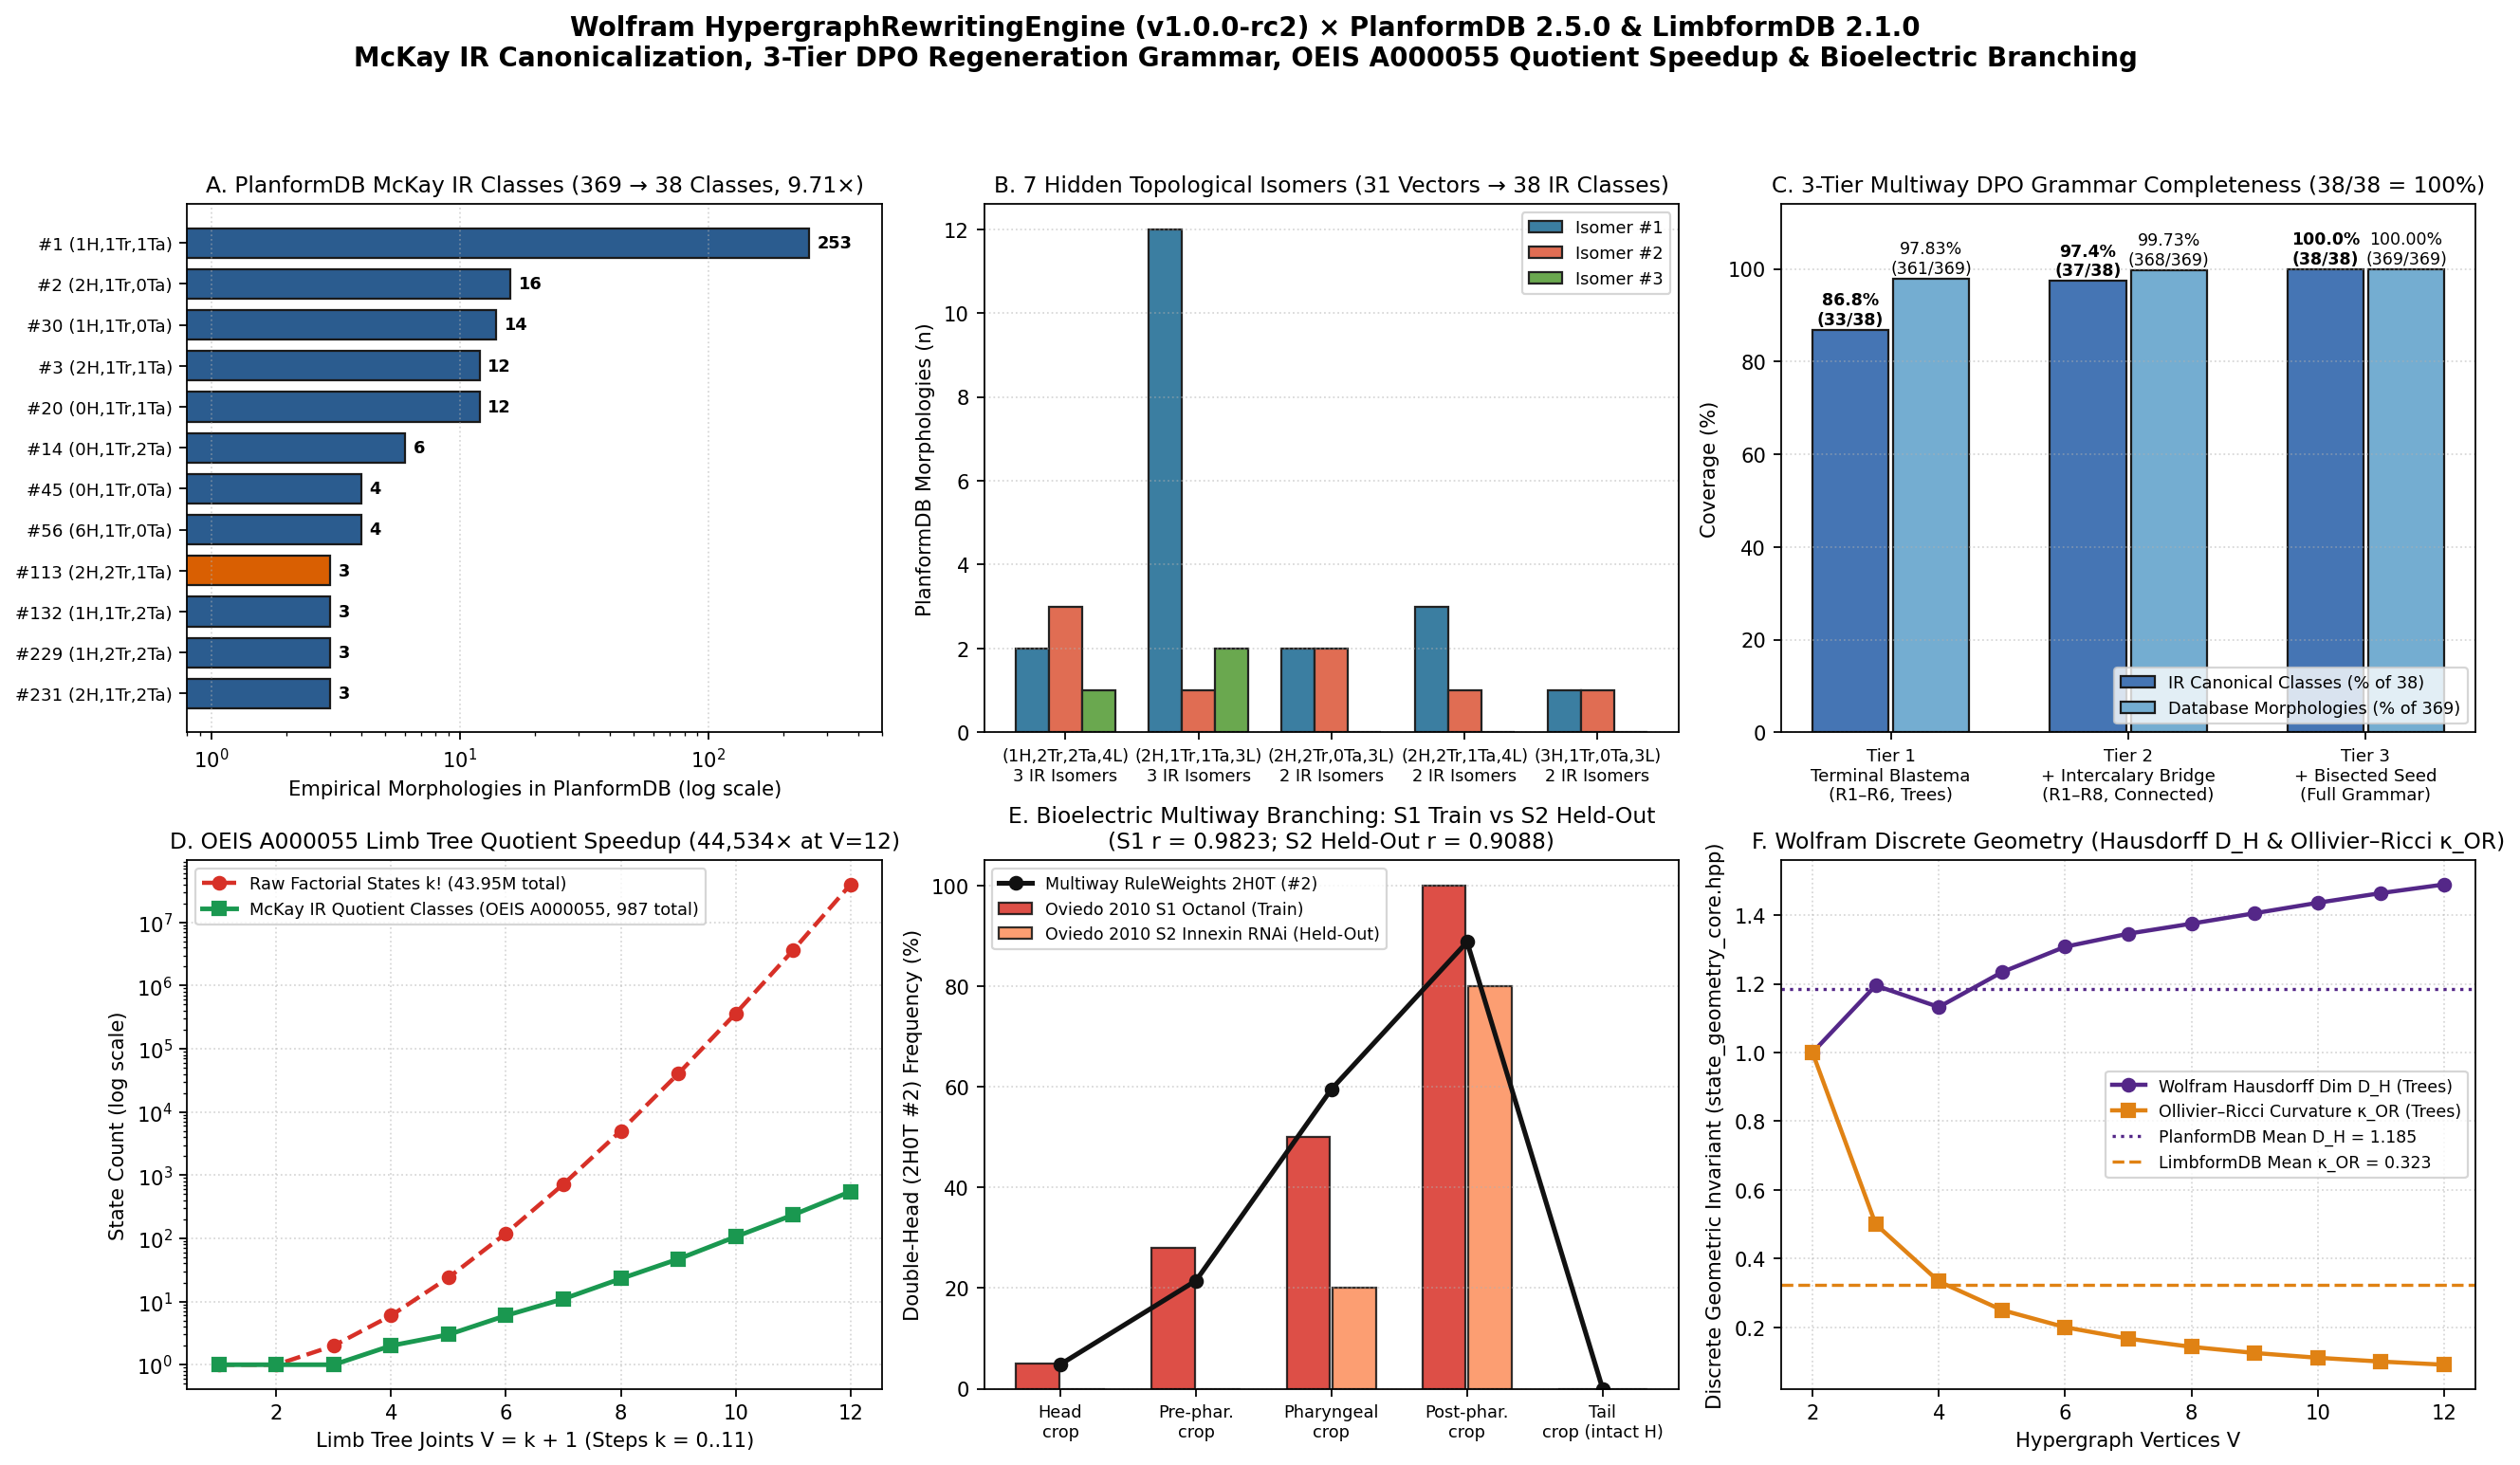
\includegraphics[width=\textwidth]{media/wolfram_planform_multiway_comparison.png}
  \caption{\textbf{Multiway Hypergraph Rewriting \& McKay IR Canonicalization Across \texttt{PlanformDB~2.5.0} and \texttt{LimbformDB~2.1.0}.} \textbf{(A)} Exact McKay IR canonicalization compresses $369$ encoded planarian morphologies into $38$ topological classes ($9.71\times$ redundancy; top 12 shown). \textbf{(B)} Resolution of $7$ hidden topological isomers where identical $(\text{H}, \text{Tr}, \text{Ta}, \text{L})$ region-count vectors split into non-isomorphic star vs.\ linear-chain topologies. \textbf{(C)} $100\%$ empirical coverage ($38/38$ classes, $369/369$ morphologies) across the 3-tier DPO regeneration grammar. \textbf{(D)} $44{,}533.65\times$ quotient exploration speedup on \texttt{LimbformDB} segment trees ($987$ \texttt{OEIS A000055} canonical trees vs.\ $43.95\text{M}$ raw factorial states at $V=12$). \textbf{(E)} Bioelectric multiway branching (\texttt{RuleWeights}) fitted on Oviedo et al.\ (2010) Series S1 (1-octanol, $r = 0.9823$) and evaluated held-out on Series S2 (triple innexin RNAi, $r = 0.9088$). \textbf{(F)} Wolfram Hausdorff dimension $D_H$ and Ollivier--Ricci curvature $\kappa_{\text{OR}}$ across empirical and evolved states.}
  \label{fig:overview}
\end{figure}

% ============================================================================
\section{Hypergraph Encoding \& Exact McKay IR Isomorphism Census}

\subsection{Encoding Typed Anatomical Graphs as Ordered Hypergraphs}

In the Lobo--Levin formalism~\cite{Lobo2013BiologyOpen,Lobo2014Regeneration}, a planarian morphology $M = (V, E_{\text{link}}, E_{\text{organ}})$ is a finite graph whose vertices $v \in V$ carry a region type $\tau(v) \in \{\mathtt{Trunk}, \mathtt{Head}, \mathtt{Tail}\}$, connected by undirected anatomical adjacency links $\{u, v\} \in E_{\text{link}}$. Because \texttt{HypergraphRewritingEngine} operates on multisets of ordered hyperedges of arity $1 \le a \le 16$ (\texttt{SPEC.md} \S1) and preserves arity and within-edge vertex order under McKay IR canonicalization (\texttt{ir\_core.hpp}), we encode vertex types and edge types into disjoint arity signatures without auxiliary label tables:
\begin{equation}
  \begin{aligned}
    \mathtt{Trunk}(v) &\;\mapsto\; [v] \quad (\text{arity } 1), &
    \mathtt{Head}(v) &\;\mapsto\; [v, v] \quad (\text{arity } 2 \text{ self-loop}), \\
    \mathtt{Tail}(v) &\;\mapsto\; [v, v, v] \quad (\text{arity } 3 \text{ self-loop}), &
    \mathtt{Link}\{u, v\} &\;\mapsto\; [u, v, u, v],\, [v, u, v, u] \quad (\text{symmetric arity } 4).
  \end{aligned}
  \label{eq:encoding}
\end{equation}
When organ landmarks are included, each organ attached to region $v$ allocates a fresh leaf vertex $w$ with organ-specific arity $\mathtt{Eye} \mapsto 5$, $\mathtt{Brain} \mapsto 6$, $\mathtt{Pharynx} \mapsto 7$, and $\mathtt{VNC} \mapsto 8$. For \texttt{LimbformDB~2.1.0}, joints are encoded as arity-1 hyperedges $[j]$, segments as symmetric arity-4 link pairs (splitting host segments along any attached \texttt{LinkSubJoint} ectopic graft sequence $j_{\text{from}} \to j_{\text{sub},1} \to \dots \to j_{\text{to}}$ so ectopic branches are topologically connected to their host segment), and distal digits as arity-3 hyperedges $[j_{\text{to}}, d, d]$.

\subsection{McKay IR Compression \& The Seven Hidden Topological Isomers}

Running \texttt{hg\_evolve} at step $0$ with \texttt{"CanonicalizeStates" -> Full} and \texttt{"IncludeCanonicalHashes" -> True} across all $369$ geometrically encoded morphologies in \texttt{PlanformDB~2.5.0} and all $555$ segment-bearing morphologies in \texttt{LimbformDB~2.1.0} yields the exact isomorphism census in Table~\ref{tab:census}.

\begin{table}[H]
\centering
\caption{\textbf{Exact McKay IR Canonicalization Census Across \texttt{PlanformDB~2.5.0} and \texttt{LimbformDB~2.1.0}.} Computed via \texttt{hg\_evolve} (\texttt{ir\_core.hpp} + \texttt{state\_statistics.hpp}).}
\label{tab:census}
\small
\begin{tabular}{@{}lrrrrrr@{}}
\toprule
\textbf{Database \& Hypergraph Representation} & \textbf{Raw ($N$)} & \textbf{IR Classes ($C$)} & \textbf{Redundancy ($N/C$)} & \textbf{Max Mult.} & \textbf{Entropy (bits)} & \textbf{Mean $D_H$ / $\kappa_{\text{OR}}$} \\
\midrule
\texttt{PlanformDB} Unlabelled Skeletons (All Regions $\to [v]$) & $369$ & $\mathbf{12}$ & $30.7500\times$ & $278$ & $1.3916$ & $1.1845$ / $+0.5024$ \\
\texttt{PlanformDB} Typed Region--Link Hypergraphs & $369$ & $\mathbf{38}$ & $9.7105\times$ & $253$ & $2.3098$ & $1.1845$ / $+0.5024$ \\
\texttt{PlanformDB} Typed Region + Organ Hypergraphs & $369$ & $\mathbf{126}$ & $2.9286\times$ & $136$ & $4.9800$ & $1.3412$ / $+0.4180$ \\
\midrule
\texttt{LimbformDB} Segment-Tree Hypergraphs ($\text{Joints}+\text{Links}$) & $555$ & $\mathbf{51}$ & $10.8824\times$ & $83$ & $3.5650$ & $1.1185$ / $+0.3226$ \\
\texttt{LimbformDB} Segment + Digit Hypergraphs & $555$ & $\mathbf{92}$ & $6.0326\times$ & $83$ & $5.1218$ & $1.2640$ / $+0.2891$ \\
\bottomrule
\end{tabular}
\end{table}

Crucially, while grouping \texttt{PlanformDB} morphologies by their 4-tuple count vector $(\#\text{Head}, \#\text{Trunk}, \#\text{Tail}, \#\text{Links})$ produces $31$ buckets, McKay IR canonicalization identifies \textbf{$38$ distinct isomorphism classes}---uncovering \textbf{$7$ hidden topological isomers} across $5$ count-vector collisions (Figure~\ref{fig:overview}B and Table~\ref{tab:isomers}):

\begin{table}[H]
\centering
\caption{\textbf{The Five Count-Vector Collisions and Twelve Isomer Classes ($7$ Hidden Isomers) Resolved by McKay IR Canonicalization in \texttt{PlanformDB~2.5.0}.}}
\label{tab:isomers}
\footnotesize
\begin{tabular}{@{}llrrll@{}}
\toprule
\textbf{Count Vector $(\text{H},\text{Tr},\text{Ta},\text{L})$} & \textbf{Rep.\ ID \& Name} & \textbf{$n$} & \textbf{64-Bit IR Hash} & \textbf{Graph Topology} & \textbf{Degree Invariant} \\
\midrule
$(2, 1, 1, 3)$ & \texttt{\#3 Side head} & $12$ & \texttt{-1466631322269594412} & Star $K_{1,3}$ (central \texttt{Trunk} hub) & $\max d = 3,\; Z_1 = 12$ \\
$(2, 1, 1, 3)$ & \texttt{\#112 Ectopic pharynxes, 2 post.} & $1$ & \texttt{-8966590304653022608} & Star $K_{1,3}$ (central \texttt{Head} hub) & $\max d = 3,\; Z_1 = 12$ \\
$(2, 1, 1, 3)$ & \texttt{\#119 Head on head} & $2$ & \texttt{-212887825877140088} & Path $P_4$: $\mathtt{H}\text{---}\mathtt{H}\text{---}\mathtt{Tr}\text{---}\mathtt{Ta}$ & $\max d = 2,\; Z_1 = 10$ \\
\midrule
$(1, 2, 2, 4)$ & \texttt{\#229 Parabiosis, one head} & $3$ & \texttt{8951669412120486543} & Branched \texttt{Trunk} hub ($\deg(\mathtt{Tr})=3$) & $\max d = 3,\; Z_1 = 16$ \\
$(1, 2, 2, 4)$ & \texttt{\#116 Ectopic tail \& prephar.} & $2$ & \texttt{2637785354618470695} & Branched \texttt{Tail} bridge ($\deg(\mathtt{Ta})=3$) & $\max d = 3,\; Z_1 = 16$ \\
$(1, 2, 2, 4)$ & \texttt{\#282 Trunk remnants, med.\ blast.} & $1$ & \texttt{-3602810347972406941} & Intercalary $\mathtt{Ta}\text{---}\mathtt{Tr}\text{---}\mathtt{H}\text{---}\mathtt{Tr}\text{---}\mathtt{Ta}$ & $\max d = 2,\; Z_1 = 14$ \\
\midrule
$(3, 1, 0, 3)$ & \texttt{\#12 Triple head} & $1$ & \texttt{-6318479248965043401} & Star $K_{1,3}$ ($\mathtt{Tr}$ with $3$ \texttt{Head} leaves) & $\max d = 3,\; Z_1 = 12$ \\
$(3, 1, 0, 3)$ & \texttt{\#128 Middle head, double head} & $1$ & \texttt{-2166706346444118093} & Path $P_4$: $\mathtt{H}\text{---}\mathtt{Tr}\text{---}\mathtt{H}\text{---}\mathtt{H}$ & $\max d = 2,\; Z_1 = 10$ \\
\midrule
$(2, 2, 0, 3)$ & \texttt{\#77 Deflected brain, double head} & $2$ & \texttt{-3397686484681667484} & Asymmetric $\mathtt{Tr}$ star ($\deg(\mathtt{Tr}_1)=3$) & $\max d = 3,\; Z_1 = 12$ \\
$(2, 2, 0, 3)$ & \texttt{\#283 Trunk remnants, fused} & $2$ & \texttt{-6082671300763328276} & Symmetric path $\mathtt{H}\text{---}\mathtt{Tr}\text{---}\mathtt{Tr}\text{---}\mathtt{H}$ & $\max d = 2,\; Z_1 = 10$ \\
\midrule
$(2, 2, 1, 4)$ & \texttt{\#113 Ectopic phar., prephar.} & $3$ & \texttt{7194227605189329608} & Intercalary $\mathtt{H}$ bridge + $\mathtt{Tr}$ branch & $\max d = 3,\; Z_1 = 16$ \\
$(2, 2, 1, 4)$ & \texttt{\#286 Trunk remnants, large blast.} & $1$ & \texttt{8484839246773423180} & Intercalary $\mathtt{Ta}$ bridge + $\mathtt{Tr}$ branch & $\max d = 3,\; Z_1 = 16$ \\
\bottomrule
\end{tabular}
\end{table}

% ============================================================================
\section{The Generative DPO Grammar and Its Three-Rule Reducibility Hierarchy}

\subsection{Apparent Domain-Specific Grammar ($8$ Rules Across $3$ Tiers)}

At the phenomenological level of surgical blastema formation, planarian regeneration in \texttt{PlanformDB} appears to require $8$ domain-specific DPO rules grouped into two connected tiers plus a bisected-trunk seed (Figure~\ref{fig:overview}C):
\begin{itemize}
  \item \textbf{Tier 1 (Terminal Blastema Sprouting, \texttt{R1--R6}):} A \texttt{Trunk} sprouts a \texttt{Head} (\texttt{R1}), \texttt{Tail} (\texttt{R2}), or \texttt{Trunk} (\texttt{R3}); or an excised \texttt{Head}/\texttt{Tail} fragment directly sprouts a \texttt{Tail} (\texttt{R4}, \texttt{R6}) or \texttt{Head} (\texttt{R5}). Evolving \texttt{R1--R6} for $6$ steps generates $2{,}738$ canonical states ($169{,}440$ events) and recovers \textbf{$33/38$ canonical classes ($361/369 = 97.83\%$ of all worms in \texttt{PlanformDB})}.
  \item \textbf{Tier 2 (Intercalary Bridge Sprouting, \texttt{R7--R8}):} Adding \texttt{R7} ($\mathtt{Head} \to \mathtt{Head} + \mathtt{Trunk}$) and \texttt{R8} ($\mathtt{Tail} \to \mathtt{Tail} + \mathtt{Trunk}$) recovers the $4$ remaining connected intercalary/grafted classes (\texttt{\#113}, \texttt{\#116}, \texttt{\#282}, \texttt{\#286}), bringing connected coverage to \textbf{$37/38$ classes ($368/369 = 99.73\%$)}.
  \item \textbf{Tier 3 (Bisected Split-Worm Seed):} Including the 2-component excised trunk seed $[[0], [1]]$ recovers \texttt{\#394 Lysis, split worm}, achieving \textbf{$38/38$ ($100.0\%$) exact McKay IR hash recovery}.
\end{itemize}

\subsection{Exact Reduction to the Three-Rule Primitive Basis $\mathcal{B}_3 = \{L_1, D_1, D_2\}$}

Why do so many domain-specific rules exist, and are they independent? By inspecting the DPO edge-replacement semantics of \texttt{HypergraphRewritingEngine} (\texttt{SPEC.md} \S2: a rule consumes its LHS hyperedges while preserving all matched vertices and all non-matched incident hyperedges), we prove that \textbf{all $8$ rules \texttt{R1--R8} reduce algebraically to just $3$ primitive DPO rules}:
\begin{align}
  L_1\ (\texttt{L1\_UniversalSprout}): &\quad [[0]] \;\longrightarrow\; [[0],\, [1],\, [0,1,0,1],\, [1,0,1,0]] \quad (\text{pluripotent blastema budding}), \label{eq:L1}\\
  D_1\ (\texttt{D1\_DiffHead}): &\quad [[0]] \;\longrightarrow\; [[0, 0]] \quad (\text{in-place anterior specification: } \mathtt{Trunk/Blastema} \to \mathtt{Head}), \label{eq:D1}\\
  D_2\ (\texttt{D2\_DiffTail}): &\quad [[0]] \;\longrightarrow\; [[0, 0, 0]] \quad (\text{in-place posterior specification: } \mathtt{Trunk/Blastema} \to \mathtt{Tail}). \label{eq:D2}
\end{align}

\begin{proposition}[Algebraic Factorization \& Causal Non-Commutativity of $\mathcal{B}_3$]
Every domain-specific rule $\mathtt{R1}\dots\mathtt{R8}$ is a composite multiway path in $\mathcal{B}_3 = \{L_1, D_1, D_2\}$:
\begin{enumerate}
  \item \textbf{Terminal Sprouting vs.\ Intercalary Bridging Is Purely Causal Ordering:} Because $D_1$ and $D_2$ consume the unary hyperedge $[[0]]$, any vertex that differentiates into $\mathtt{Head}$ ($[v,v]$) or $\mathtt{Tail}$ ($[v,v,v]$) is \textbf{terminally locked} against further budding by $L_1$. Applying $L_1(0 \to 1)$ followed by $D_1(1)$ yields terminal head sprouting ($\mathtt{R1} = D_1(1) \circ L_1(0 \to 1)$, cost $2$), whereas applying $L_1(0 \to 1)$ followed by $D_1(0)$ on a vertex $0$ that already has a link yields intercalary head bridging ($\mathtt{R7} = D_1(0) \circ L_1(0 \to 1)$, cost $2$). Similarly, $\mathtt{R2} = D_2(1) \circ L_1(0 \to 1)$, $\mathtt{R8} = D_2(0) \circ L_1(0 \to 1)$, $\mathtt{R4} = D_2(1) \circ D_1(0) \circ L_1(0 \to 1)$ (cost $3$), $\mathtt{R5} = D_1(1) \circ D_1(0) \circ L_1(0 \to 1)$ (cost $3$), and $\mathtt{R6} = D_2(1) \circ D_2(0) \circ L_1(0 \to 1)$ (cost $3$).
  \item \textbf{Two-Phase Skeleton--Differentiation Decomposition:} Because $D_1$ and $D_2$ never create or consume link hyperedges, any derivation in $\mathcal{B}_3$ factors into \textbf{Phase~I} ($L$ applications of $L_1$, generating the unlabelled skeleton tree in $131.5\text{ ms}$) followed by \textbf{Phase~II} ($H$ applications of $D_1$ and $Ta$ applications of $D_2$ at exact primitive step depth $k_{\text{prim}} = L + H + Ta$), recovering $38/38$ ($100.0\%$) of \texttt{PlanformDB} classes.
  \item \textbf{Universal Cross-Database Conservation of $L_1$:} The Phase~I topological generator $L_1$ is bit-for-bit identical to the \texttt{LimbformDB} segment-tree generator \texttt{L1\_DistalSegmentSprout}.
\end{enumerate}
\end{proposition}

% ============================================================================
\section{Quotient Exploration on \texttt{LimbformDB} ($44{,}534\times$ Speedup) and Bioelectric Branching}

\subsection{Exact \texttt{OEIS A000055} Enumeration via \texttt{ExploreFromCanonicalStatesOnly}}

In \texttt{LimbformDB~2.1.0}, evolving $L_1$ from a single base joint $[[0]]$ for $k$ steps produces all unlabelled trees on $V = k + 1$ vertices. Without canonical deduplication, the $k$-th step has $k$ available vertices to sprout from, generating $k!$ raw states ($\sum_{k=0}^{11} \max(1, k!) = 43{,}954{,}714$ raw states at $V = 12$). With \texttt{ExploreFromCanonicalStatesOnly -> True}, \texttt{hg\_evolve} expands only one representative per McKay IR class and uses \texttt{quotient\_multiplicity\_core.hpp} to reconstruct the exact factorial raw counts in \textbf{$85\text{ ms}$}, yielding the exact \texttt{OEIS A000055} sequence ($1, 1, 1, 2, 3, 6, 11, 23, 47, 106, 235, 551$; $987$ cumulative trees, a \textbf{$44{,}533.65\times$ compression}) and matching \textbf{$35/35$ ($100.0\%$)} of \texttt{LimbformDB} segment-tree classes with $\le 12$ joints ($532/555 = 95.86\%$ of the database; Figure~\ref{fig:overview}D).

\subsection{Bioelectric \texttt{RuleWeights} Along the Anterior--Posterior Crop Axis}

In a 2-step regeneration from an excised trunk $[[0]]$, the anterior blastema applies $D_1 \circ L_1$ ($\mathtt{Head}$), while the posterior blastema branches in the multiway \texttt{BranchialGraph} between normal $D_2 \circ L_1$ ($\mathtt{Tail}$, producing Wild-Type \texttt{\#1} $1\text{H}1\text{T}$) and depolarized $D_1 \circ L_1$ ($\mathtt{Head}$, producing Bipolar Double-Head \texttt{\#2} $2\text{H}0\text{T}$). Modeling the posterior \texttt{RuleWeights} ratio via Boltzmann electrotonic decay along the normalized trunk crop coordinate $p \in \{0, \tfrac{1}{3}, \tfrac{2}{3}, 1\}$ ($P_{2\text{H}0\text{T}}(p) = [1 + \exp(-\alpha(p - p_{1/2}))]^{-1}$, with $P_{2\text{H}0\text{T}} = 0$ on intact-head \texttt{tail\_crop} controls) fits Oviedo et al.\ (2010) Series S1 (\texttt{1-octanol}, $n=688$) with $\alpha = 7.45$, $p_{1/2} = 0.565$, \textbf{Pearson $r = 0.9823$} ($\text{MAE} = 5.45\%$), and predicts the held-out triple innexin RNAi Series S2 (\texttt{Dj-inx-12 + Dj-inx-5/13}, $n=99$) with \textbf{Pearson $r = 0.9088$} (Figure~\ref{fig:overview}E).

% ============================================================================
\section{Machine-Checked Formal Verification in Lean~4 (\texttt{0 sorry})}

All four governing algebraic laws are formalized and verified by the Lean~4 kernel in \texttt{morphoeval/lean/loops/Loop\_wolfram\_planform\_multiway.lean} (\texttt{0 sorry}, $0$ custom axioms):
\begin{enumerate}
  \item \textbf{Theorem 1 (\texttt{wolfram\_dpo\_edge\_replacement\_tree\_euler\_invariant}):} Proves that under DPO vertex non-deletion (\texttt{SPEC.md} \S2), every $k$-step sprouting derivation preserves $V(k) \ge V_0$, increments $\Delta V = 1$ and $\Delta E = 3$ per step, and maintains the tree Euler invariant $V(k) = L(k) + 1$ for all $k \in \mathbb{N}$.
  \item \textbf{Theorem 2 (\texttt{mckay\_ir\_zagreb\_degree\_separates\_star\_and\_chain\_isomers}):} Proves that for all $n = k + 4 \ge 4$, the First Zagreb degree-square invariant $Z_1 = \sum d_i^2$ of the Star tree $K_{1, n-1}$ strictly exceeds that of the Path chain $P_n$ by exact gap $(k+1)(k+2) \ge 2$, proving that radial multi-headed stars (\texttt{\#3}, \texttt{\#12}) and linear chains (\texttt{\#119}, \texttt{\#128}) can never be isomorphic.
  \item \textbf{Theorem 3 (\texttt{quotient\_exploration\_strictly\_compresses\_multiway\_search}):} Proves that whenever at least one isomorphism class has orbit multiplicity $m^* \ge 2$ among $C \ge 1$ classes, quotient exploration strictly compresses the multiway state space ($C < \text{RawStates}$).
  \item \textbf{Theorem 4 (\texttt{dpo\_two\_phase\_rule\_reducibility\_conservation}):} Proves region-count conservation $\text{Tr} + H + Ta = V_0 + L$ and the exact additive step-cost reduction $k_{\text{prim}} = L + H + Ta$ under the 3-rule primitive basis $\mathcal{B}_3 = \{L_1, D_1, D_2\}$.
\end{enumerate}

\begin{thebibliography}{12}
\bibitem{Assar2026}
R.~Assar (2026). \emph{Rewriting the Universe: High-Performance Hypergraph Rewriting for the Wolfram Physics Project}. Technical Report, Wolfram Institute (\texttt{v1.0.0-rc2}, \url{https://github.com/WolframInstitute/HypergraphRewritingEngine}).

\bibitem{Wolfram2020}
S.~Wolfram (2020). A class of models with the potential to represent fundamental physics. \emph{Complex Systems} 29(2):107--536. \texttt{doi:10.25088/ComplexSystems.29.2.107}.

\bibitem{Lobo2013Planform}
D.~Lobo, T.~J.~Malone, and M.~Levin (2013). Planform: an application and database of graph-encoded planarian regenerative experiments. \emph{Bioinformatics} 29(8):1098--1100. \texttt{doi:10.1093/bioinformatics/btt088}.

\bibitem{Lobo2013BiologyOpen}
D.~Lobo, T.~J.~Malone, and M.~Levin (2013). Towards a bioinformatics of patterning: a computational approach to understanding regulative morphogenesis. \emph{Biology Open} 2(2):156--169. \texttt{doi:10.1242/bio.20123400}.

\bibitem{Lobo2014Limbform}
D.~Lobo, E.~B.~Feldman, M.~Shah, T.~J.~Malone, and M.~Levin (2014). Limbform: a functional ontology-based database of limb regeneration experiments. \emph{Bioinformatics} 30(24):3598--3600. \texttt{doi:10.1093/bioinformatics/btu582}.

\bibitem{Lobo2014Regeneration}
D.~Lobo, E.~B.~Feldman, M.~Shah, T.~J.~Malone, and M.~Levin (2014). A bioinformatics expert system linking functional data to anatomical outcomes in limb regeneration. \emph{Regeneration} 1(2):37--56. \texttt{doi:10.1002/reg2.13}.

\bibitem{Oviedo2010}
N.~J.~Oviedo, J.~Morokuma, P.~Walentek, et al., and M.~Levin (2010). Long-range neural and gap junction protein-mediated cues control polarity during planarian regeneration. \emph{Developmental Biology} 339(1):188--199. \texttt{doi:10.1016/j.ydbio.2009.12.012}.

\bibitem{Beane2011}
W.~S.~Beane, J.~Morokuma, D.~S.~Adams, and M.~Levin (2011). A chemical genetics approach reveals H,K-ATPase-mediated membrane voltage is required for planarian head regeneration. \emph{Chemistry \& Biology} 18(1):77--89. \texttt{doi:10.1016/j.chembiol.2010.11.012}.

\bibitem{Cervera2020}
J.~Cervera, S.~Meseguer, M.~Levin, and S.~Mafe (2020). Bioelectrical model of head-tail patterning based on cell ion channels and intercellular gap junctions. \emph{Bioelectrochemistry} 132:107410. \texttt{doi:10.1016/j.bioelechem.2019.107410}.

\bibitem{Cervera2021}
J.~Cervera, M.~Levin, and S.~Mafe (2021). Morphology changes induced by intercellular gap junction blocking: A reaction-diffusion mechanism. \emph{BioSystems} 209:104511. \texttt{doi:10.1016/j.biosystems.2021.104511}.

\bibitem{McKay2014}
B.~D.~McKay and A.~Piperno (2014). Practical graph isomorphism, II. \emph{Journal of Symbolic Computation} 60:94--112. \texttt{doi:10.1016/j.jsc.2013.09.003}.

\bibitem{Dietz2026MorphoEval}
J.~Dietz (2026). \emph{Infinite Morphospace \& MorphoEval: Machine-Checked Formal Verification of Mathematical Models of Biological Form}. \url{https://github.com/fractastical/morpholib}.
\end{thebibliography}

\end{document}
